\begin{center}
\section*{\month}
\end{center}

\def\day{\textit{April 1st, 2021}}
\def\weekday{\textit{Thursday}}
\subsection*{\weekday, \day}
Today I instaled this diary. 

\def\day{\textit{April 3st, 2021}}
\def\weekday{\textit{Thursday}}
\subsection*{\weekday, \day}

I set up Android Studio and tried to install a KVM (i think it means Kernal Virtual Mashine) with \\
https://help.ubuntu.com/community/KVM/Installation\\

how to creat a android app with androidstudio \\
https://developer.android.com/training/basics/firstapp/creating-project \\ 

fundamentals how android apps works \\
https://developer.android.com/guide/components/fundamentals \\ 

How does an app get permissions for camera etc.\\ 
https://developer.android.com/guide/topics/permissions/overview\\

Activities\\
https://developer.android.com/guide/components/activities/intro-activities\\

Services\\
https://developer.android.com/guide/components/services\\

Notifications\\
https://developer.android.com/guide/topics/ui/notifiers/notifications\\

Content providers\\
https://developer.android.com/guide/topics/providers/content-providers\\

\newpage

Each Android app lives in its own security sandbox, protected by the following Android security features: \\ 
\begin{itemize}
    \item The Android operating system is a multi-user Linux system in which each app is a different user. \\
    \item By default, the system assigns each app a unique Linux user ID (the ID is used only by the system and is unknown to the app). \\
    The system sets permissions for all the files in an app so that only the user ID assigned to that app can access them. \\   
    \item Each process has its own virtual machine (VM), so an app's code runs in isolation from other apps. \\
    \item By default, every app runs in its own Linux process.  \\ 
    The Android system starts the process when any of the app's components need to be executed, \\
    and then shuts down the process when it's no longer needed or when the system must recover memory for other apps. \\
\end{itemize}

However, there are ways for an app to share data with other apps and for an app to access system services:\\ 
\begin{itemize}
    \item It's possible to arrange for two apps to share the same Linux user ID, in which case they are able to access each other's files. \\
    To conserve system resources, apps with the same user ID can also arrange to run in the same Linux process and share the same VM. The apps must also be signed with the same certificate.\\
    \item An app can request permission to access device data such as the device's location, camera, and Bluetooth connection.\\ 
    The user has to explicitly grant these permissions. For more information, see Working with System Permissions.\\
\end{itemize}

\newpage    
There are four different types of app components:\\

    Activities\\
    Services\\
    Broadcast receivers\\
    Content providers\\

\textbf{Activities}

An activity is the entry point for interacting with the user. It represents a single screen with a user interface. For example, an email app might have one activity that shows a list of new emails, 
another activity to compose an email, and another activity for reading emails. Activities can be stopped and run again. And they can be started from other apps. \\

An activity facilitates the following key interactions between system and app:\\
\begin{itemize}
    \item Keeping track of what the user currently cares about (what is on screen) to ensure that the system keeps running the process that is hosting the activity.\\
    \item Knowing that previously used processes contain things the user may return to (stopped activities), and thus more highly prioritize keeping those processes around.\\
    \item Helping the app handle having its process killed so the user can return to activities with their previous state restored.\\
    \item Providing a way for apps to implement user flows between each other, and for the system to coordinate these flows. (The most classic example here being share.)\\
\end{itemize}

\textbf{Services}

A service is a general-purpose entry point for keeping an app running in the background for all kinds of reasons.
It is a component that runs in the background to perform long-running operations or to perform work for remote processes.
A service does not provide a user interface. \\

For example, a service might play music in the background while the user is in a different app, or it might fetch data over the network without blocking user interaction with an activity.
Another component, such as an activity, can start the service and let it run or bind to it in order to interact with it.\\

\newpage

Syncing data in the background or playing music also represent two different types of started services that modify how the system handles them:\\ 
\begin{itemize}
    \item Music playback is something the user is directly aware of, so the app tells the system this by saying it wants to be foreground with a notification to tell the user about it; \\
    in this case the system knows that it should try really hard to keep that service's process running, because the user will be unhappy if it goes away.\\\\
    \item A regular background service is not something the user is directly aware as running, so the system has more freedom in managing its process. \\
    It may allow it to be killed (and then restarting the service sometime later) if it needs RAM for things that are of more immediate concern to the user.\\
\end{itemize}

Bound services run because some other app (or the system) has said that it wants to make use of the service. This is basically the service providing an API to another process. 
If one service is importent the bound service will also be important.\\

\textbf{Broadcast receivers}

A broadcast receiver is a component that enables the system to deliver events to the app outside of a regular user flow, allowing the app to respond to system-wide broadcast announcements. \\
Because broadcast receivers are another well-defined entry into the app, the system can deliver broadcasts even to apps that aren't currently running.\\
Apps can kinda communicate with broadcast reciever.\\
More commonly, though, a broadcast receiver is just a gateway to other components and is intended to do a very minimal amount of work. \\
For instance, it might schedule a JobService to perform some work based on the event with JobScheduler\\

\textbf{Content provider}

A content provider manages a shared set of app data that you can store in the file system, in a SQLite database, on the web, or on any other persistent storage location that your app can access. 
Through the content provider, other apps can query or modify the data if the content provider allows it.\\

To the system, a content provider is an entry point into an app for publishing named data items, identified by a URI scheme. 
Thus an app can decide how it wants to map the data it contains to a URI namespace, handing out those URIs to other entities which can in turn use them to access the data. 
There are a few particular things this allows the system to do in managing an app:
\begin{itemize}
    \item Assigning a URI doesn't require that the app remain running, so URIs can persist after their owning apps have exited. 
    The system only needs to make sure that an owning app is still running when it has to retrieve the app's data from the corresponding URI.
    \item These URIs also provide an important fine-grained security model. 
    For example, an app can place the URI for an image it has on the clipboard, but leave its content provider locked up so that other apps cannot freely access it. 
    When a second app attempts to access that URI on the clipboard, 
    the system can allow that app to access the data via a temporary URI permission grant so that it is allowed to access the data only behind that URI, but nothing else in the second app.
\end{itemize}
Content providers are also useful for reading and writing data that is private to your app and not shared.\\
A content provider is implemented as a subclass of ContentProvider and must implement a standard set of APIs that enable other apps to perform transactions. 
For more information, see the Content Providers developer guide.\\\\

%=============================================================================================================================================

A unique aspect of the Android system design is that any app can start another app’s component. 
For example, if you want the user to capture a photo with the device camera, 
there's probably another app that does that and your app can use it instead of developing an activity to capture a photo yourself. 
You don't need to incorporate or even link to the code from the camera app. 
Instead, you can simply start the activity in the camera app that captures a photo. 
When complete, the photo is even returned to your app so you can use it. To the user, it seems as if the camera is actually a part of your app.\\

When the system starts a component, it starts the process for that app if it's not already running and instantiates the classes needed for the component. 
For example, if your app starts the activity in the camera app that captures a photo, that activity runs in the process that belongs to the camera app, not in your app's process. 
Therefore, unlike apps on most other systems, Android apps don't have a single entry point (there's no main() function).\\

Because the system runs each app in a separate process with file permissions that restrict access to other apps, your app cannot directly activate a component from another app. 
However, the Android system can. To activate a component in another app, deliver a message to the system that specifies your intent to start a particular component. 
The system then activates the component for you.


\def\day{\textit{April 5st, 2021}}
\def\weekday{\textit{Thursday}}
\subsection*{\weekday, \day}

I started a dictionary


\def\day{\textit{April 11st, 2021}}
\def\weekday{\textit{Thursday}}
\subsection*{\weekday, \day}

I'm imforming myself about git.
https://www.youtube.com/watch?v=2sjqTHE0zok

\newpage

\def\day{\textit{April 12st, 2021}}
\def\weekday{\textit{Thursday}}
\subsection*{\weekday, \day}


So right now i'm kindy angry at my self because I didn't look up what I have to learn to programm a App. Like i have to know the basics of Android UI and Android (I guess its a Ligary.)\\
So now i'm on \\
for a complete tutorial how to make a app\\
https://abhiandroid.com/createandroidapp/ \\

for a quick tutorial how to make a calculater\\
https://abhiandroid.com/createandroidapp/create-calculator-app \\
i just played around a little bit and relized XML is not that hard, just I just have to remeber alot \\
/home/liquid/AndroidStudioProjects/calculater\\\\

learning Android \\
https://abhiandroid.com/programming/ \\

Android UI,Layout and Material Design Tutorial, Examples And Code\\
https://abhiandroid.com/ui/



\def\day{\textit{April 13st, 2021}}
\def\weekday{\textit{Thursday Simon}}
\subsection*{\weekday, \day}
We arranged that we work independent till Sunday (18.4.21) on research for the GUI. So that in the end we can exchange our knowlege. 
and we arranged that we work on Hello world 

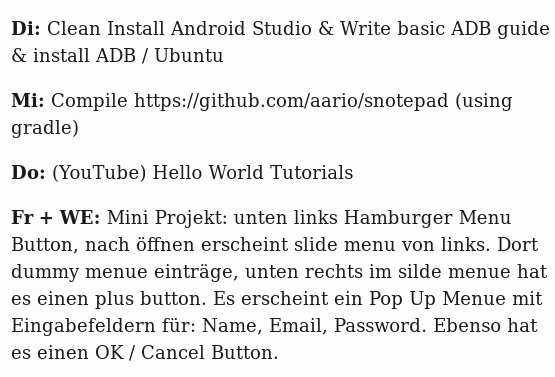
\includegraphics[width=.8\textwidth]{media/WochenPlan13.4.jpeg}


\def\day{\textit{April 13st Noah, 2021}}
\def\weekday{\textit{Thursday}}
\subsection*{\weekday, \day}

I successfully installed both NDK and SDK on my Arch Linux Desktop PC. Now Android Studio won't crash on startup.


\def\day{\textit{April 14st Simon, 2021}}
\def\weekday{\textit{Thursday}}
\subsection*{\weekday, \day}
Apps provide multiple entry points

Android apps are built as a combination of components that can be invoked individually. For example, an activity is a type of app component that provides a user interface (UI).

The "main" activity starts when the user taps your app's icon. You can also direct the user to an activity from elsewhere, such as from a notification or even from a different app.

Other components, such as broadcast receivers and services, allow your app to perform background tasks without a UI.

After you build your first app, you can learn more about the other app components at Application fundamentals.
Apps adapt to different devices

Android allows you to provide different resources for different devices. For example, you can create different layouts for different screen sizes. The system determines which layout to use based on the screen size of the current device.

If any of your app's features need specific hardware, such as a camera, you can query at runtime whether the device has that hardware or not, and then disable the corresponding features if it doesn't. You can specify that your app requires certain hardware so that Google Play won't allow the app to be installed on devices without them.

After you build your first app, learn more about device configurations at Device compatibility overview. 
https://developer.android.com/training/basics/firstapp

Installed java 8 so i can compile the build.gradle file but for this wasn't enough time

\def\day{\textit{April 14st Noah, 2021}}
\def\weekday{\textit{Wednesday}}
\subsection*{\weekday, \day}

I sucessfully managed to compile the app \url{https://github.com/aario/snotepad} on Arch Linux using the \texttt{jdk8-openjdk} package.\\

Also I installed Ubuntu, so I could use the same environment as Simon.\\

I wrote the adb guide \url{https://noahvogt.com/resources/adb-guide.html} and corrected all the errors Simon pointed out to me.

\def\day{\textit{April 15st Simon, 2021}}
\def\weekday{\textit{Thursday}}
\subsection*{\weekday, \day}

I finally could compile the testapp to an apk file. 


\newpage
\def\day{\textit{April 19st Noah, 2021}}
\def\weekday{\textit{Monday}}
\subsection*{\weekday, \day}

\begingroup
\setlength{\intextsep}{10pt}
\setlength{\columnsep}{15pt}

\begin{wrapfigure}{l}{8cm}
\centering
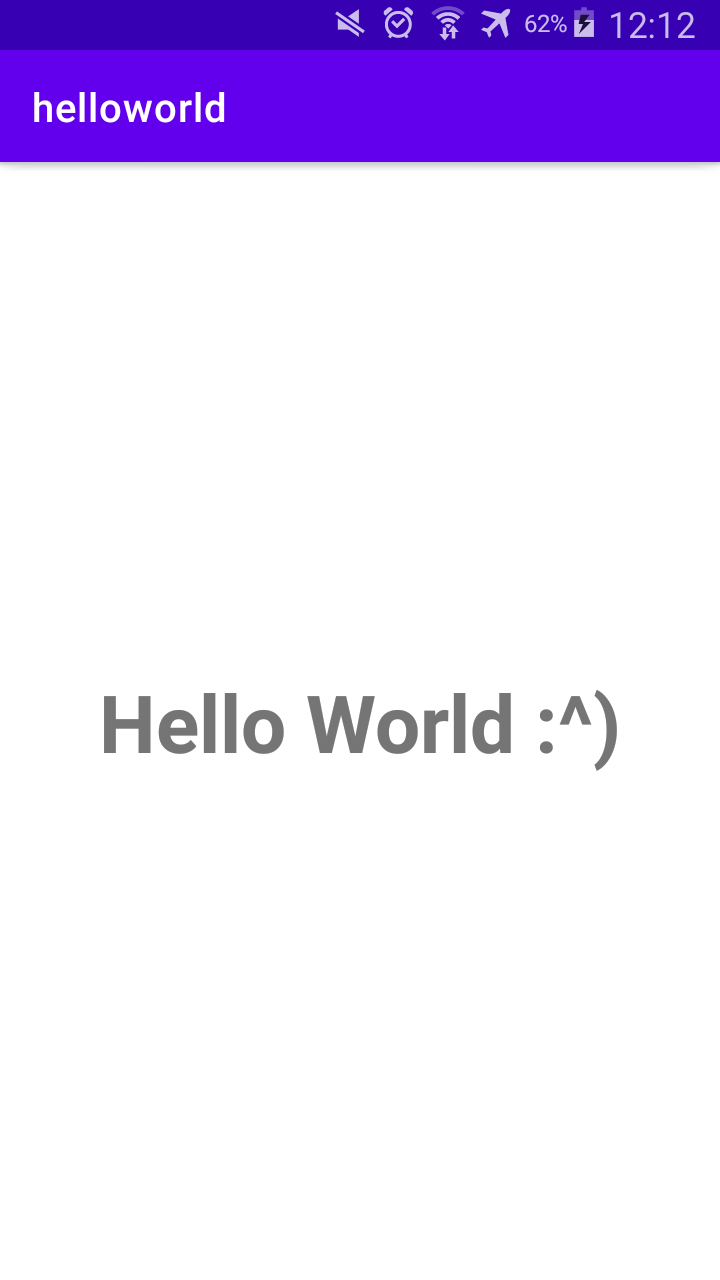
\includegraphics[scale=.15]{media/hello-world-app-noah-screenshot}
\caption{Hello World}
\end{wrapfigure}

I updated the adb guide as requested from Simon to include the Activation of the Android USB Debbing. I also made some additional changes.\\

I made a Hello World Program, installed it via adb on my phone and captured this screenshot of it also using adb.\\

Also, I made a private github repo \url{https://github.com/noahvogt/mini-project}.\\

On there it is planned to work on features in seperate branches that will only be merged into the master branch, when they are in a usable state.

\endgroup

\vspace{4cm}
\begingroup
\setlength{\intextsep}{10pt}
\setlength{\columnsep}{15pt}

\begin{wrapfigure}{r}{8cm}
\centering
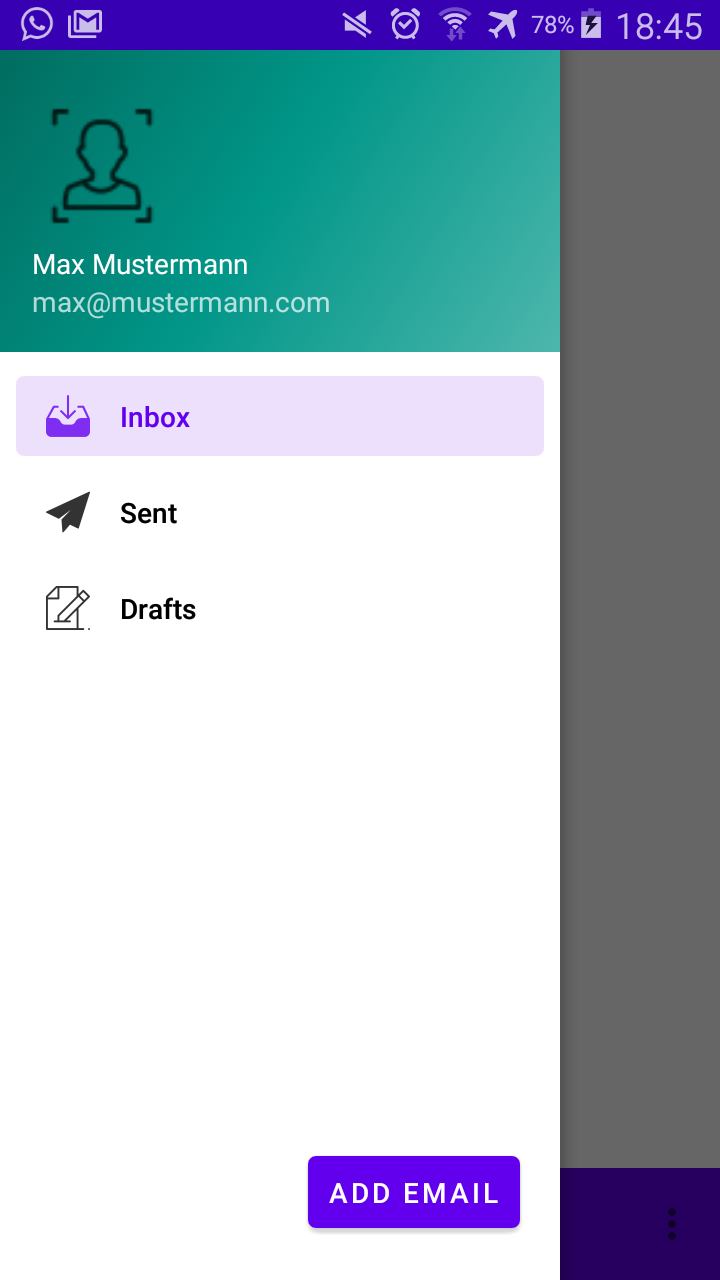
\includegraphics[scale=.15]{media/drawer}
\caption{Drawer Navigation Menu}
\end{wrapfigure}
I then made the app more functional, so that you have a base GUI with a drawer, a menu in the bottom and in the drawer navigation menu you can tap on the «Add Email» Button and a popup window will come up asking you for name, email and password. Even the save and cancel button work. Now we only need a functionality to save this information to a string somewhere in the main activity.\\

For this I created a new branch called \texttt{newemail-popup}.


\endgroup
\newpage

\def\day{\textit{April 19st Simon, 2021}}
\def\weekday{\textit{Monday}}
\subsection*{\weekday, \day}
Interfaces specify what a class must do and not how. It is the blueprint of the class.
An Interface is about capabilities like a Player may be an interface and any class implementing Player must be able to (or must implement) move(). So it specifies a set of methods that the class has to implement.
If a class implements an interface and does not provide method bodies for all functions specified in the interface, then the class must be declared abstract.
A Java library example is Comparator Interface. If a class implements this interface, then it can be used to sort a collection.

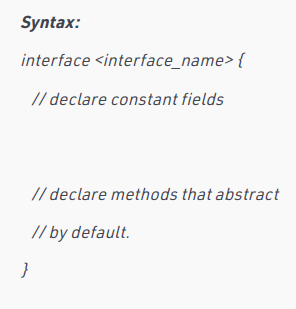
\includegraphics[width=.4\textwidth]{media/SyntactsInterface.png}


\def\day{\textit{April 20 Noah, 2021}}
\def\weekday{\textit{Wednesday}}
\subsection*{\weekday, \day}

I continued my work on \texttt{newemail-popup} and looked up more ways how we  could implement this. I am not sure yet, what we will go for right now.\\

I also applied the GNU General Public License v3 on all upstream branches. I think it is useful to choose a free license right away, instead of waiting too long.

\def\day{\textit{April 21 Noah, 2021}}
\def\weekday{\textit{Wednesday}}
\subsection*{\weekday, \day}

After Simon mentioned to me that he couldn't install the unsigned release apk from our build, I tried it myself. It turned out you would have to sign this jar/apk, before your android phone will accept to install it.\\

So I searched ways how to do it outside of anroid studio, just on the command line. I did try out some software projects and shell scripts, but none of them worked. ADB told me now, that instead of no certificates, I would have inconsistent ones.\\

So I have successfully wasted 1 - 3 hours on finding out how to sign a apk. But I consider this issue not relevant right now, and in the worst case will be solvable by just using android studio. So I decided to ignore this issue for now and just use the debug apk for now.
